\section{Experimental Analysis for Prediction Algorithms}
\label{sec:experiment_design}


In this section we examing the performance of the multiband placement algorithms. We study the algorithms on regular grid topologies and then real topologies in different scenarios distinguished by propagation and legal white bands.

J. Robinson has validated the capacity calculation in ~\cite{robinson2008adding} through TFA network measurement and calculation. Multiband scenario has the same calculation and physical meanings with single band described in ~\cite{robinson2008adding}.
The actual throughput values are able to be mapped to real network.

\subsection{Performance in Regular Grid}
\label{subsec:regulargrid}

First we study the performance of the two algorithms, ~\emph{Multiband MinHopCount, Multiband MinContention} presented in Section ~\ref{sec:algorithms}.
For all experiments, we consider an 802.11b system with the single band link wireless throughput assumed to be 6Mbps.
All mesh node locations are fixed and gateways can be installed on any mesh node.
We compar the algorithms against a FIXME placement strategy.

The topology for experiment in this sub-section is a placement of $7 \times 7$ regular grid. A mesh node communicates directly with at most 4 neighbors and contents with all two hop neighbors in a single band.






\subsection{In-Field Data Collection}
\label{exp:datacollection}
Next we will introduce the analysis based on in-field experiment. We collect data on a off-shelf multiband platform and smartphone platform. The potential gateway nodes locations are from existing mesh network TFA and Google Wifi. 
The two algorithms in 4 different kind of environment with propagation and white bands are analyzed in the following.

We introduce the experimental set up for ~\emph{Multiband Mesh Network}. There are two set of experiments for characteristic leveraging of multiple scenarios presented ~\ref{sec:propagation}. 
One is the ~\emph{Local Multiband Measurement} grab propogation information across bands; the other is ~\emph{WiEye} helps to find the propogation relationship of multiple cities. The methodology to process the data is also introduced.

\subsubsection{Local Multiband Measurement}
To discover the propagation diversity, we measure 4 different bands, 450MHz, 900MHz, 2.4GHz, and 5.8GHz on our off-shelf multiband platform. 
The measurement platform is made of Gateworks 2358 with GPS, Smartbridge 450MHz radio, Ubiquite XR2, XR5, and XR9 radios. 
The software on the platform is Linux based Openwrt with several third party applications such as Iperf, TCPdump.
We bring 2 of this platform on cars and run Iperf at the transmitter with GPS records to generate traffic on the four bands simultaneously sending through the radios on the platform.
The TCPdump running on the receiver side sniffs the packets and report the SNR with GPS information.

% Assume the pathloss exponent the same across bands or different pathloss exponent????

% Measurement processing
Comparing the GPS records on both side help to grab the distance between the transmitter and receiver with time stamps. The SNR and distance could be synchronized according to the time stamps.
The propagation relationship of four different bands across different environment could be found through the curve fitting. 

% WiEye measurements
\subsubsection{WiEye Measurement}
% FIXME add Wieye intro from Web
WiEye is an Android application help users to measure the ~\emph{Access Point} signal strength provided by SMU ~\emph{Wireless Networks Group} for free. It also help ~\emph{Wireless Networks Group} collecting measurement data of signal strength to leverage the propogation characteristics on large scale ~\cite{meikle2012global}.
Due to the hardware limitation, most of the cellphones can only work on 2.4GHz, most of the measurement data is on 2.4GHz. 
The data from WiEye helps to get the propogation of a city in 2.4GHz and according our 2.4GHz multiband measurements, we map the propogation in other bands of the cities. 

% Find AP location methodology
An issue of the WiEye measurement is that the ~\emph{Wifi Access Points} are unknown of the users. To overcome the issue, we propose a methodology to estimate the ~\emph{Access Point} through multiple measurement.
The ~\emph{Path Loss Exponent} varies from 2 to 5 in different environment ~\cite{camp2006measurement}. 
First we grab measurements in the same area, pull out their location information and signal strength information.
Then, we assume the area have a small ~\emph{Path Loss Exponent}. If there are ~\emph{Access Points} at the location of the users, their connectivity circle click will cover the actual ~\emph{Access Point}. The area covered by the most virtual click is believed to be the plane contain the ~\emph{Access Point}.
Third, we increase the ~\emph{Pass Loss Exponent} to decrease the click of the virtual click getting close to the ~\emph{Access Point} in the plane of the last step. We iteratively repeat the process to narrow the possible location of the ~\emph{Access Point} till there are only two virtual click cover the same location in the previous step plane. 
Then the location is believed as the ~\emph{Access Point}.

Base upon the estimation, the distance from the ~\emph{Access Point} to the users could be calculated and mapping to the SNR for propagation estimation.

FIXME{Add diagram to describe the process}

\subsubsection{Data Processing}
First we leverage the propagation exponent from the WiEye data set. Since WiEye WiFi measurement only focus on ISM 2.4GHz with GPS data, from the GPS we can learn the environment of the location from Google map. We map the WiEye single band measurement to our local multiband measurement to estimate the propagation characteristics in other bands.


\begin{figure}
%\vspace{-0.0in}
\centering
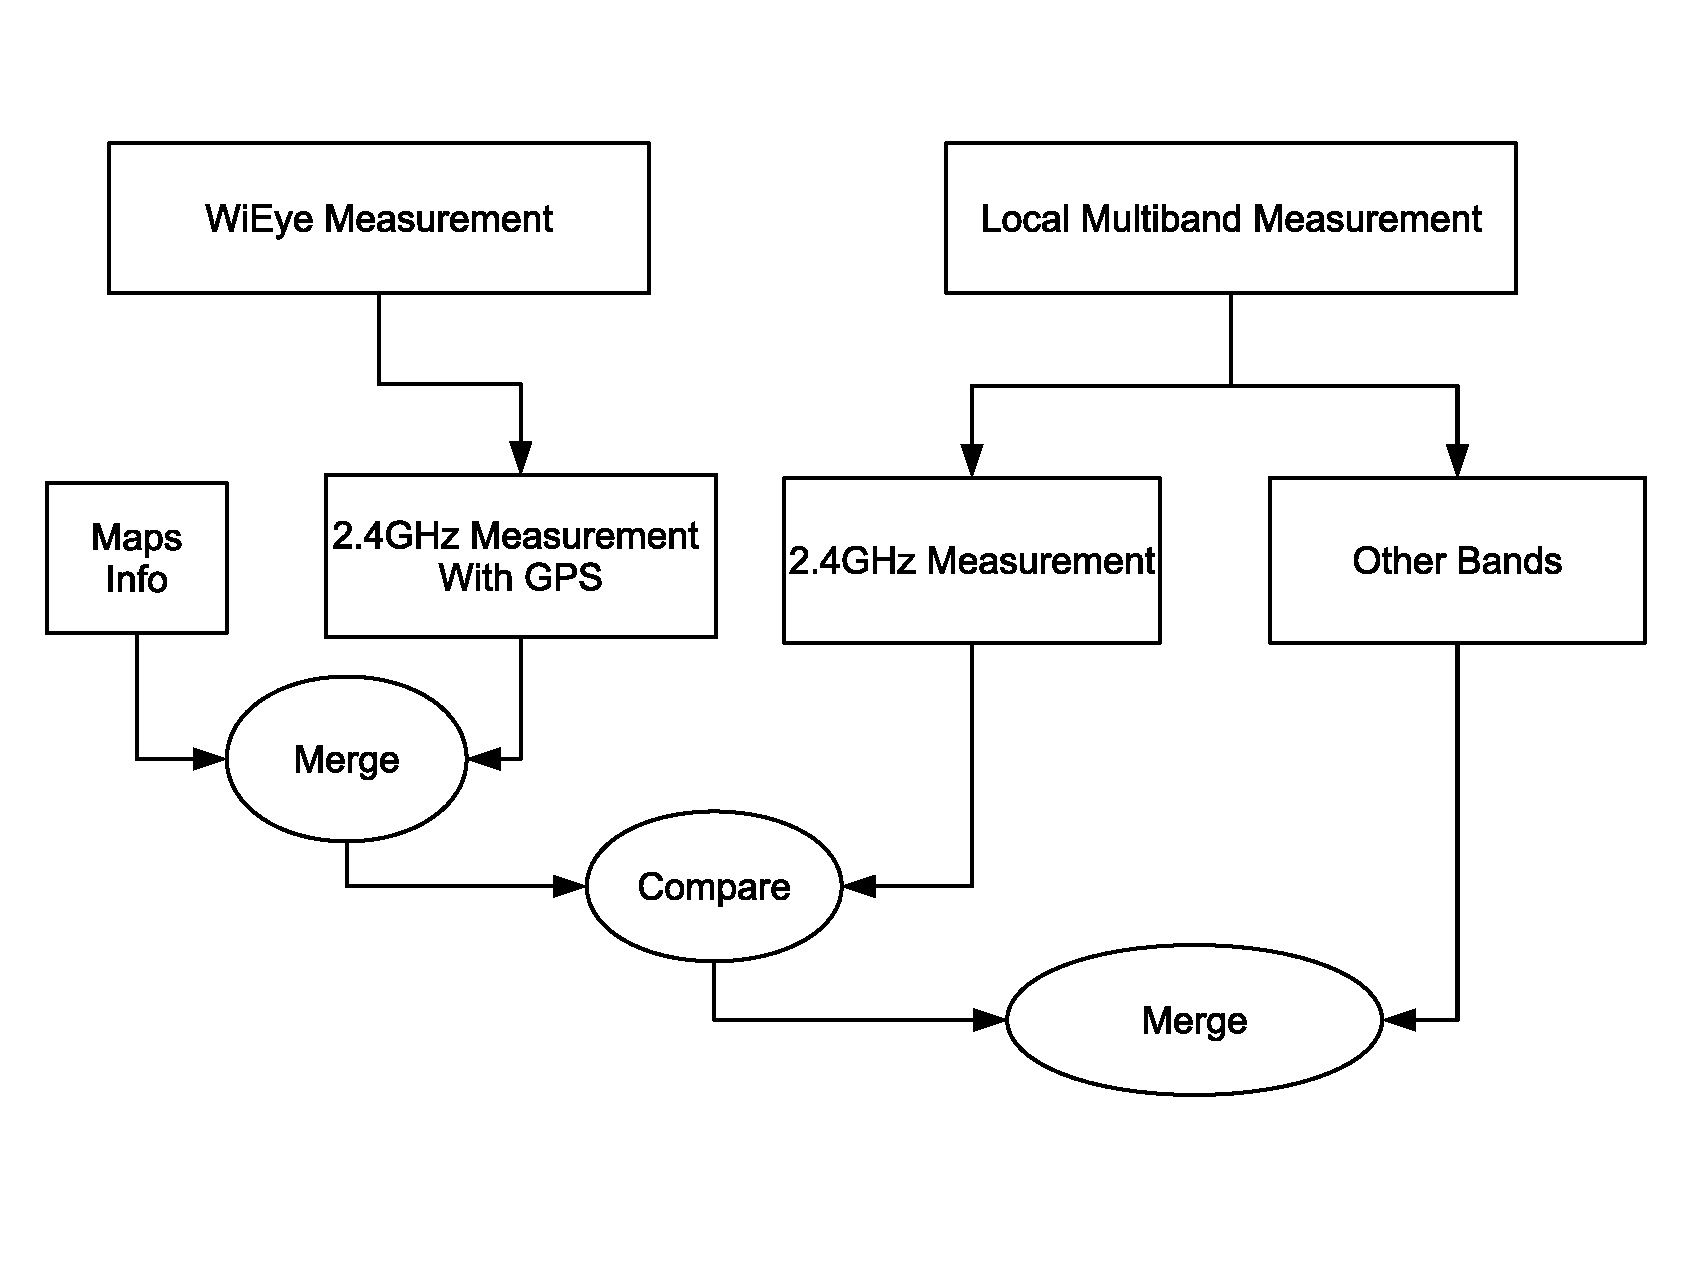
\includegraphics[width=74mm]{figures/wieye_process}
\vspace{-0.1in}
\caption{Data Merge Process}
\label{fig:wieye_process}
%\vspace{-0.0in}
\end{figure}

After the processing step, we can grab the propagation in different environment even in multiple cities. Based on the measured data, we investigate the performance of the algorithms in different scenario.
% Scenario cities analysis, experimental set up of different propagation/channel bandwidth

\subsubsection{Real-World Topologies}
We consider the placement algorithms on the topologies of FIXME currently deployed mesh networks:FIXME
For each topology, we fix a number of already installed gateways and focus on upgrading with new gateways.
The in-field nodes locations are involved in the experiment.

First, we begin with four known FIXME gateways and place additional capacity points in the network assuming the propagation characteristics are the same in the area.


Then we split the network covered area as different regions according to the geological information and FCC regulation and evaluate the algorithms performance.







